Since the system uses a Client-Server architecture, our software will have to run on two different pieces of hardware. First off, we have the clients - these are not required to be computation heavy machines. They are required to run Windows, and should be able to connect to the Internet. 
The server on the other hand, should be fairly quick machines, and have a pretty fast internet connection. The server will also run windows, and should be able to run operations offline such as matching appointments or taking backup copies. How this will be implemented in practice is yet to be determined. 


The different responsibilities of the server and client are as follows:
The Server:
\begin{itemize}
	\item Storing all data
	\item Backing up data
	\item Running our LuckyMatchFinder algorithm
	\item Authorizing the clients requests
\end{itemize}
The Client:
\begin{itemize}
	\item Keeping the local users credentials
	\item Synchronizing the local calendar with the server
	\item Saving changes when in a offline state, and later sending them to the server
	\item Providing the user with an easy-to-access UI
\end{itemize}

\begin{center}
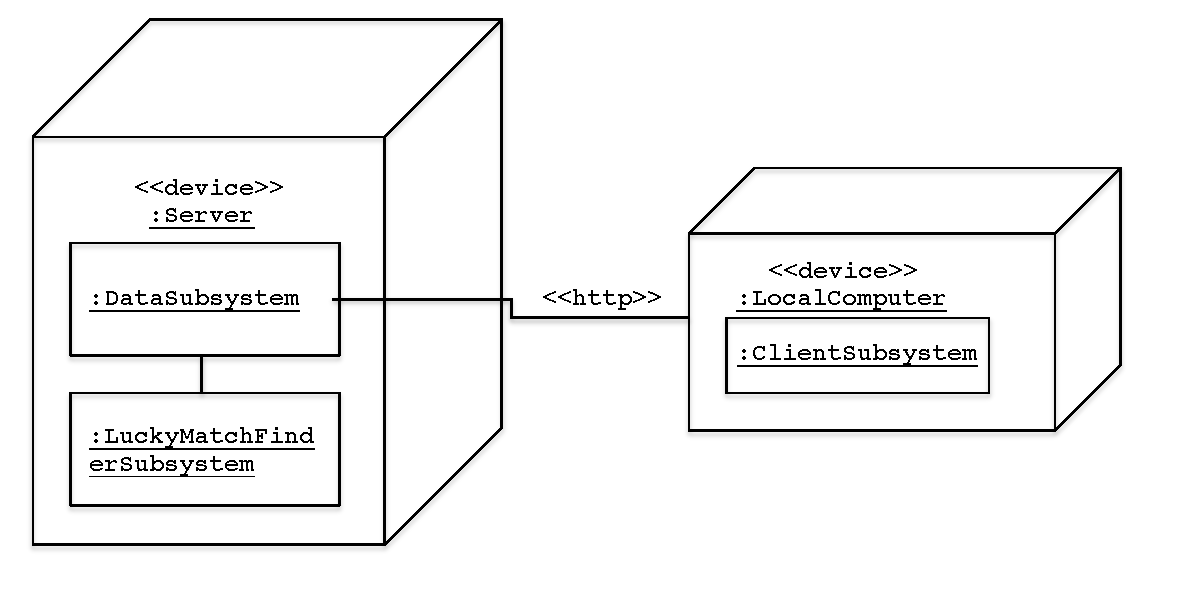
\includegraphics[scale=.8]{sections/hardwaremapping.pdf}
\end{center}

On the server side we will use the subsystem Datahandler to stay connected to the clients through a http-connection. The Client will use the model-subsystem to stay connected to the server. The clients will be logged on locally with after an authorization from the server.
The servers DataHandler will function as a wrapper class around a SQL-database, through which it will load and save data after request from the client or the LuckyMatchFinder algorithm. 

If a client for some reason should lose connection to the server, it will be able to save the changes locally instead, and will upon reconnection to the server, synchronize these changes with it. We might want to always save changes locally, but have yet to figure out the exact pros and cons, but this isn't plan yet. The clients model-subsystem uses a bridge pattern to apply the different data handling interfaces, which are assigned though a Strategy pattern which uses an Abstract Factory pattern to create the different data manager classes. The Client will also be able to synchronize with Google Calendar as a secondary server - that is, it will not replace our server, but rather work as a supplement for the user. 
